\section{Applications}
\label{sec:apps}

In Section~\ref{sec:motivating-examples}, we characterized four
applications and explained why they cannot be accommodated satisfactorily
in the status-quo web architecture. We then described the COWL system's
new browser primitives. We now close the loop by demonstrating how
to build the aforementioned applications with the COWL primitives.

\subsection{Encrypted Document Editor}

The key feature needed by an encrypted document editor is symmetric
confinement, where two mutually distrusting scripts can each confine
the other's use of data they send one another. Asymmetrically
conferring COWL privileges on the distrusting components is the key to
realizing this application.

\begin{figure}
\centerline{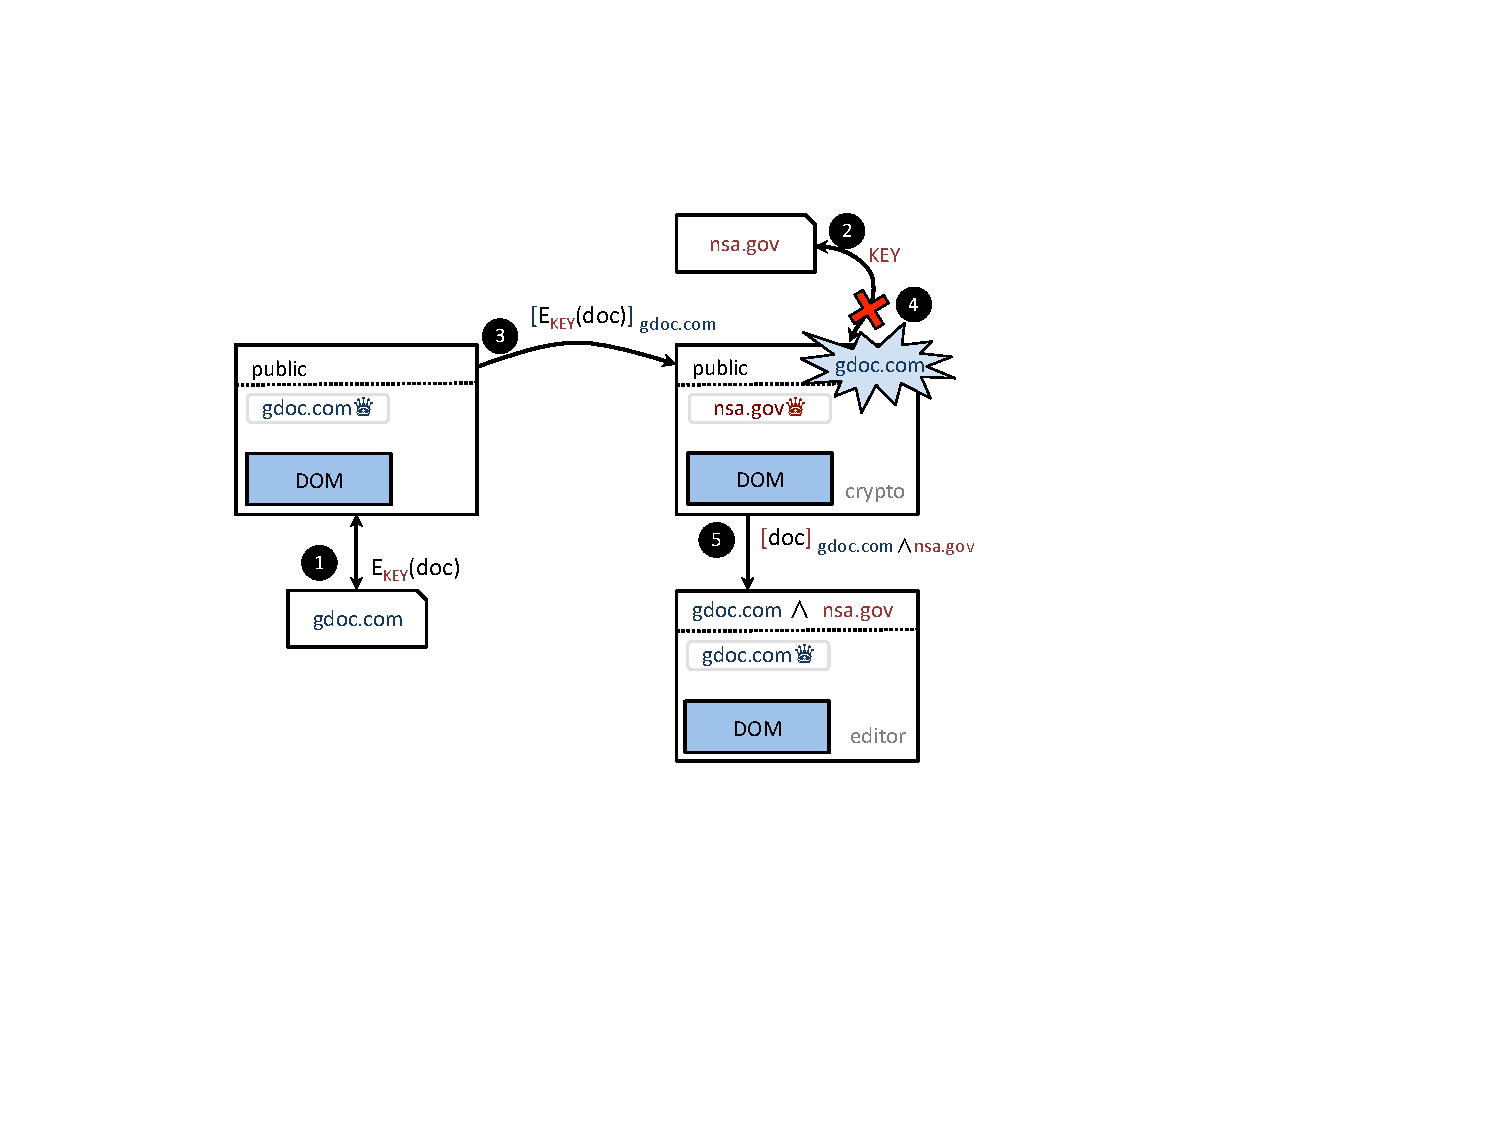
\includegraphics[width=\columnwidth]{editor}}
\caption{\label{fig:editor} Encrypted document editor architecture.}
\end{figure}

Figure~\ref{fig:editor} depicts the architecture for an encrypted
document editor. The editor has three components: a component which
has the user's Google Documents credentials and communicates with the
server (\https{gdoc.com}), the editor proper (also \https{gdoc.com}),
and the component that performs encryption (\https{nsa.gov}). COWL
provides privacy as follows: if \https{nsa.gov} is honest, then COWL
ensures that the clear text of the user's document is not leaked to
any origin. If only \https{gdoc.com} is honest, then \https{gdoc.com}
may be able to recover cleartext (\emph{e.g.,} the encryptor may have
used the null cipher), but the encryptor should not be able to
exfiltrate the cleartext to anyone else.

How does execution of the encrypted document editor proceed?
%
Initially, \https{gdoc.com} downloads (1) the encrypted document from
Google's servers.
%
As the document is encrypted, it opens an iframe to
\https{nsa.gov}, with initial label 
\js|public| so it can communicate with the \https{nsa.gov} server and
download the private key (2) which will be used to decrypt the document.
%
Next, it sends the encrypted document as a labeled Blob, with the label
\dcLabelS{\https{gdoc.com}}{} (3); the iframe unlabels the Blob and
raises its label (4) so it can decrypt the document.
%
Finally, the iframe passes the decrypted document (labeled as
\dcLabelS{\https{gdoc.com} $\land$ \https{nsa.gov}}{}) to a new iframe (5) which
implements the editor proper.

To save the document, these steps proceed in reverse: the editor sends
a decrypted document to the encryptor (5), which encrypts it with the
private key.  Next, the critical step occurs: the encryptor exercises
its privileges to send a labeled blob of the encrypted document which
is \emph{only} labeled \dcLabelS{\https{gdoc.com}}{} (3).  Since the
encryptor is the only compartment with the \https{nsa.gov} privilege,
all documents must pass through it for encryption before being sent
elsewhere; conversely, it itself cannot exfiltrate any data, as it is
confined by \https{gdoc.com} in its label.

Note that this design permits the user to verify that Google Documents
appropriately loaded the encryptor: without it, displaying the
decrypted text would be impossible. However, when a new document is
being created, the encryptor iframe must be placed in a separate
pop-up window, so that the user can verify that encryption has been
enabled.\footnote{This architecture might be desirable in any case to
  prevent phishing.}
\Red{I still don't get how the user verifies this.}

We have implemented a password manager atop COWL that lets users
safely store passwords on third-party web-accessible storage. We elide
its detailed design in the interest of brevity, and note only that it
operates similarly to the encrypted document editor.
%% In the interest of brevity, we do not discuss the architecture of the
%% \sys{} password manager; this application allows users to safely store
%% their passwords on third-party storage provides such GoogleDocs. We
%% only remark that it operates on very similar principles to the
%% encrypted document editor.

\subsection{Third-Party Mashup}
\label{sec:apps-mashup}

\begin{figure}
\centerline{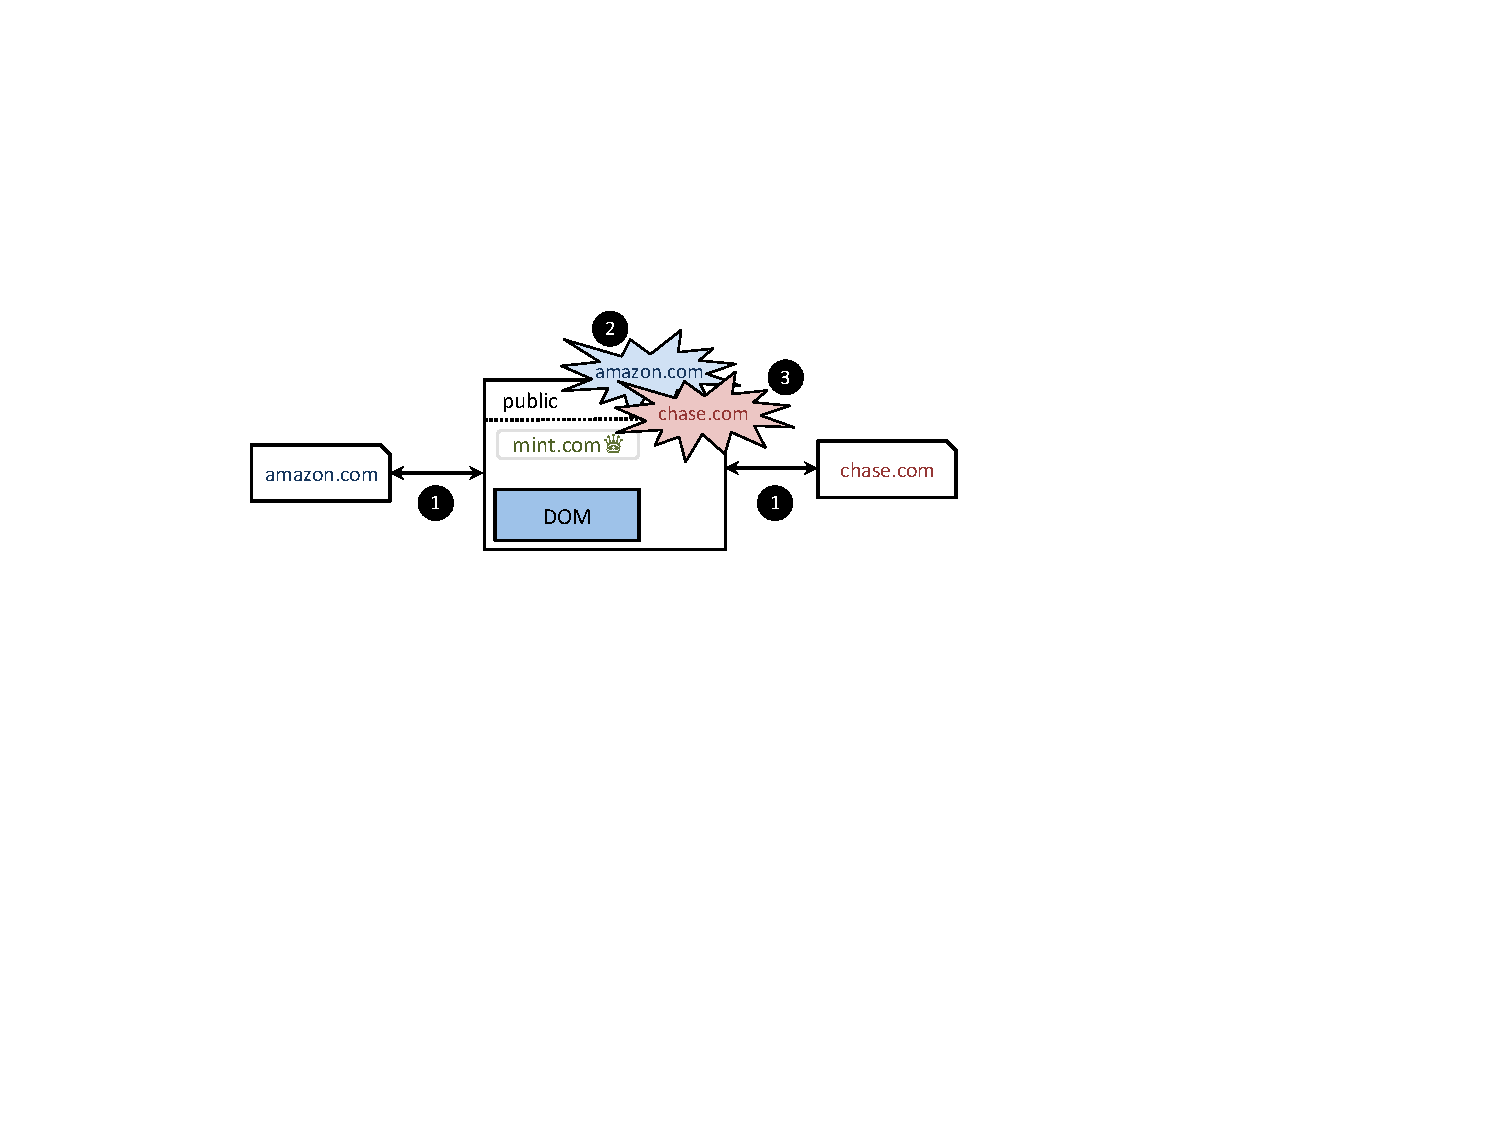
\includegraphics[width=\columnwidth]{mashup}}
\caption{\label{fig:mashup} Third-party mashup under \sys{}.}
\end{figure}
Labeled XHR as composed with CORS is central to COWL's support for
third-party mashups.
%
Today's CORS policies are DAC-only, such that a server must either
allow another origin to read its data and fully trust that origin not
to disclose the data, or deny the other origin access to the data
altogether. Under COWL, however, a server could CORS-whitelist a
foreign origin to permit that origin to read its data, and by setting
a label on its response, be safe in the knowledge that COWL would
appropriately confine the foreign origin's scripts in the browser.
 
Figure~\ref{fig:mashup} depicts an application that reconciles a
user's Amazon purchases and bank statement.
%
Here, Chase and Amazon respectively expose read-only APIS for bank
statements and purchase histories that whitelist known applications'
origins, such as \https{mint.com}, but set MAC labels on responses.
%
(As discussed in Section~\ref{sec:discussion}, with MAC in place, COWL
allows users to otherwise augment CORS by whitelisting foreign origins
on a per-origin basis.)
%
% The rest is very simple.
%
The mashup makes requests to both web sites using labeled XHR (1)
to receive the bank statement and
purchase history as labeled Blobs.
%
Once all of the information is received, the mashup unlabels it and
raises its context's label accordingly (2--3); doing so restricts
communication to the web at large.

Note that in contrast to when solely using CORS, by setting MAC labels
on responses, Chase and Amazon need not trust Mint to write bug-free
code---COWL confines the Mint code to ensure that it cannot
arbitrarily leak bank statements or purchase histories. As we discuss
in Section~\ref{sec:discussion}, however, a malicious Mint application
could potentially leak data through covert channels.  We emphasize
that COWL nevertheless offers a significant improvement over the
status quo, in which, \emph{e.g.,} users give their login credentials
to Mint, and thus not only trust Mint to keep their bank statements
confidential, but also not to steal their funds!

\subsection{Untrusted Third-Party Library}
\label{sec:apps-third-party}

\begin{figure}
\centerline{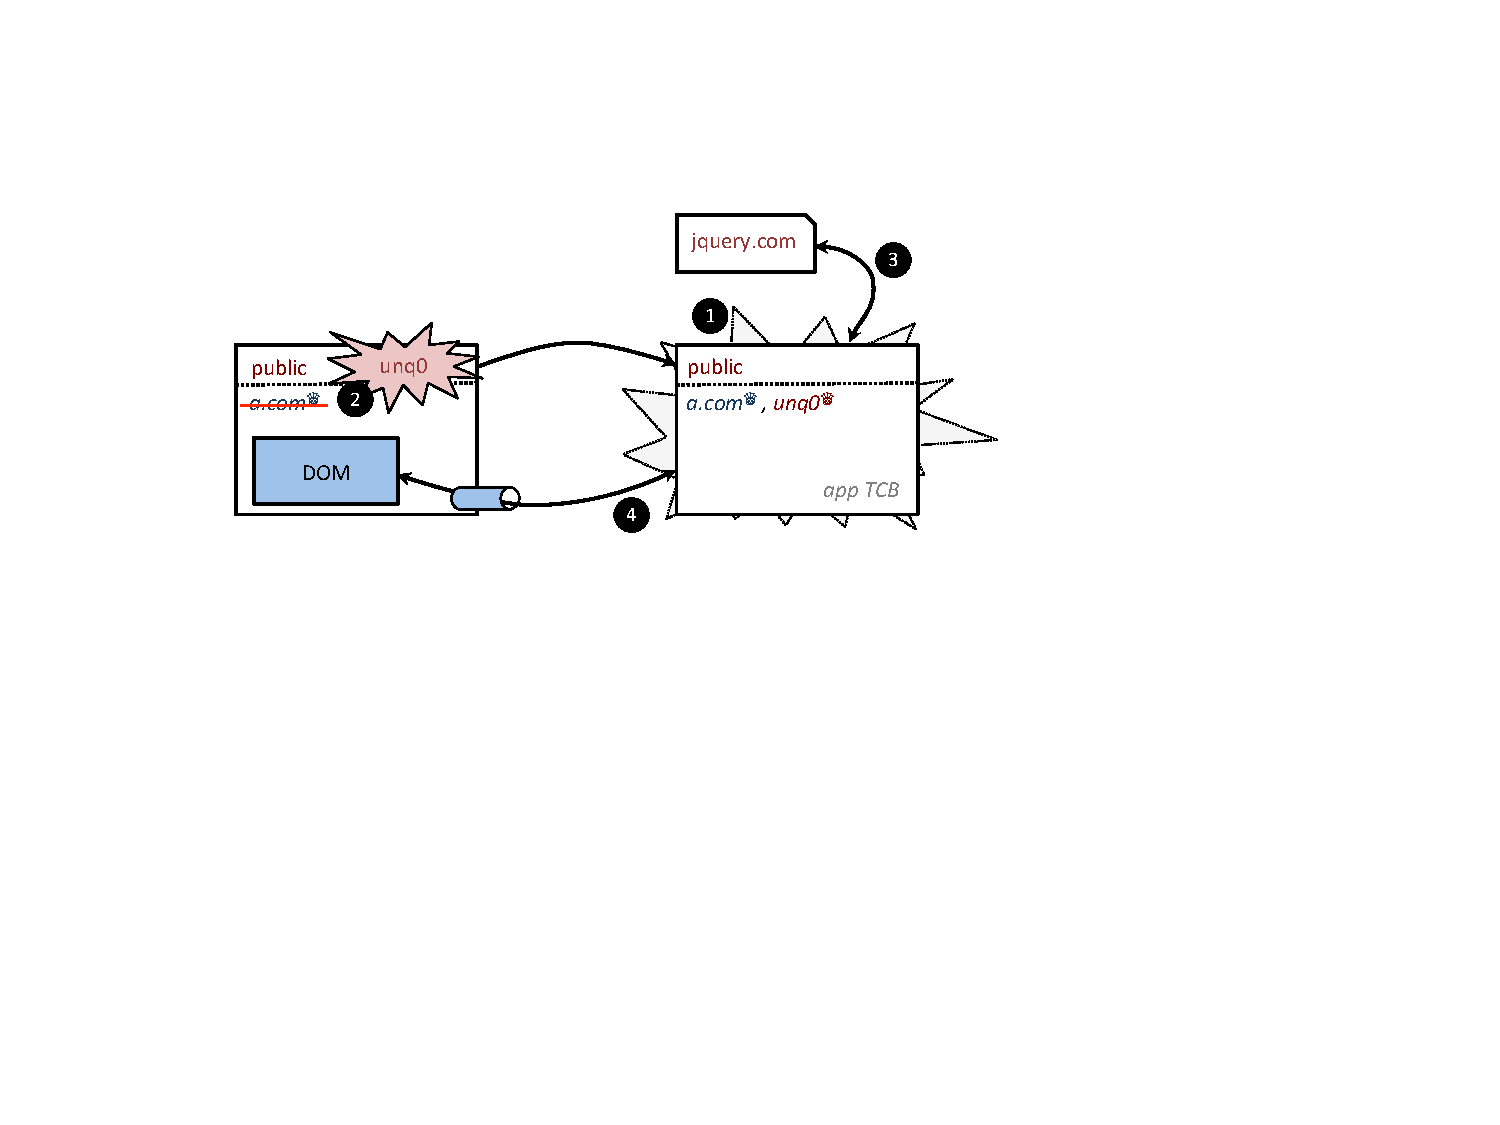
\includegraphics[width=\columnwidth]{jquery}}
\caption{\label{fig:jquery} Privilege separation and library
confinement.}
\end{figure}

COWL can confine tightly coupled untrusted third-party libraries like
jQuery by delegating privileges to a trusted context and subsequently
dropping them from the main page. In doing so, COWL completely
confines the main page, and ensures that it can only communicate with
the trusted and unconfined context.

Figure~\ref{fig:jquery} shows how to use COWL to confine the untrusted
jQuery library referenced by a web page. The goal is to establish a
separate DOM worker with the \https{a.com} privilege, while the main
browsing context runs jQuery in confined fashion---without privileges
or the ability to talk to the network. Initially the main browsing
context holds the \https{a.com} privilege. The page generates a fresh
origin \https{unq0} and spawns a DOM worker (1), delegating it both
privileges. The main context then drops its privileges and raises its
label to \dcLabelS{\https{unq0}}{} (2). Finally, the trusted worker
downloads jQuery (3) and injects the script content into the main
context's DOM (4).  When the library is loaded, the main context
becomes untrusted, but also fully confined. As the trusted DOM worker
holds both privileges, it can freely modify the DOM of the main
context, as well as communicate with the wider web. One may view
this DOM worker as a \emph{firewall} between the page proper (with the
untrusted library) and the rest of the world.
